\chapter{Marco Teórico}
% ***********************************************************************************

En el proceso de comunicación se tiene que además del emisor, el receptor y el mensaje, existe el canal, el cual para la propagación de las ondas electromagnéticas corresponden al aire o bien, a un cable conductor. Estas son usadas para transmitir información en forma de señales que en comunicaciones, viajan por distintos medios, cables de cobre, fibra óptica o enlaces de microondas, entre otros.\\

Sin embargo, la información, considerando el volumen de datos que viajan por las redes, obedece un orden, que en redes de datos se conoce como modelo OSI.\\

\newpage
\textbf{Modelo OSI}\\

Es un modelo que sirve de referencia para los protocolos que operan en las distintas capas que componen este modelo. Es un estándar desarrollado en 1980 por la ISO que establece un ordenamiento por el cual deben regirse los datos al moverse.\\

\underline{Este modelo consta de siete capas}\\

Físico, Enlace, Red, Transporte, Sesión, Presentación, Aplicación.

Donde cada nivel realiza una función concreta, y se separa de los adyacentes por interfaces conocidas, sin que le concierna ningún otro aspecto del total de la comunicación.  Las capas que participan de los modelos estudiados son las que se detallan a continuación:

\begin{itemize}

\item{\textbf{Capa Física}

Corresponde a las capa que guarda relación con la conexión, es decir, con la forma en que se conecta el dispositivo a la red y la transmisión, esto es a cómo se transmiten los datos. Entre sus funciones, está el establecer cuál o cuáles son los medios por los cuales viaja la señal y el normar las características materiales y eléctricas de los componentes.\\
}

\item{
\textbf{Capa de Enlace}\\
Esta capa representa para efectos de lo que se pretende investigar y eventualmente desarrollar, la capa que hace posible el seguimiento, pues se encarga de la transferencia de información entre la capa de red y la capa física. Y para ello se vale de tramas que le dotan al dispositivo una dirección \ac{MAC} lo que le permite hacer control de flujo, detección y corrección de errores.\\

Es de esta capa que los IPS, se valen, como es el caso de el algoritmo de trilateración en donde se establece la conexión a un AP, se hace la identificación del dispositivo a través de la dirección MAC y luego el posterior cálculo.\\
}
\end{itemize}

\newpage

\textbf{Medio No Guiado}\\

Corresponde a los medios por los cual viajan las ondas electromagnéticas y que en este caso, corresponden a dispositivos que se valen de antenas para propagarlas.\\

\textbf{Router}

Un router inalámbrico es un dispositivo que además de la función de router, sirve de punto de acceso, es decir, permite que los dispositivos inalámbricos se conecten a la red. En las funciones de router, este dispositivo direcciona los datos que provienen desde y hacia los dispositivos conectados a la red y que compartan la misma conexión de red por las distintas interfaces que la compongan, permitiendo que estos se comuniquen entre sí.\\

Todas las conexiones realizadas en la red inalámbrica se hacen dentro de lo que se denomina, para cuando se usa este tipo de redes, una red de infraestructura inalámbrica y es sobre esta que los dispositivos se comunican entre si e interactúan con la red exterior.\\

Es en esta parte donde el router recibe, desde el dispositivo móvil, solicitudes del tipo \textsc{ICMPv6}, que son un tipo de solicitudes conocidas como \ac{IRDP}  o Protocolo de descubrimiento de enrutador de internet y que son un tipo de solicitudes del protocolo \ac{ICMP} o Protocolo de control de mensajes de internet que se encargan de establecer la conexión con el router. Del tipo de mensajes ICMP existen dos tipos:\\

\begin{itemize}
\item{\textit{ICMP Router Solicitation Message:} Este tipo de mensajes es enviado desde un equipo a cualquiera de los routers que se hallen en la LAN para avisar que se encuentran en presencia de esta red. Básicamente, avisan que podrían eventualmente desear conectarse.}
\item{\textit{ICMP Router Advertisement Message}: Es enviado por el router en la LAN para anunciar la IP disponible para rutear.}\\
\end{itemize}

\begin{figure}[h!]
\centering
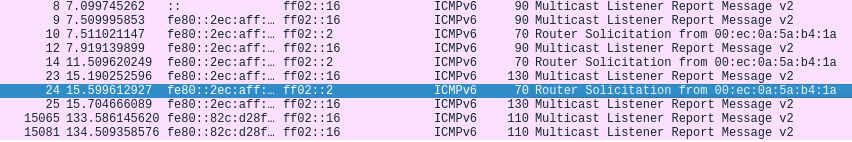
\includegraphics[scale=0.5]{./imagenes/IRDP}
\caption{Captura en Wireshark de solicitudes IRDP}
\label{fig:IRDP}
\end{figure}

Finalmente, se anuncian mediante una solicitud de establecimiento de conexión donde el router recibe la MAC del dispositivo, entre otros datos, y establece la conexión si la autenticación fue exitosa.\\


\begin{figure}[h!]
\centering
		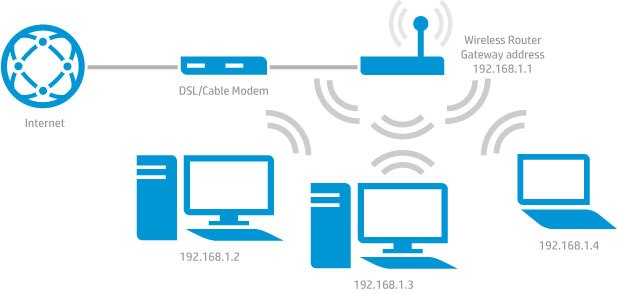
\includegraphics[scale=0.5]{./imagenes/ap}
		\label{fig:access_point}
		\caption{Ejemplo de red de infraestructura inalámbrica$^{\ref{fig:paginaHP}}$}
\end{figure}

De ser exitosa, el router, mediante el protocolo \ac{DHCP}, asigna desde el número limitado de direcciones IP que el \ac{ISP} entrega al cliente, una IP que enlaza esta dirección con la MAC del usuario estableciendo así la conexión. Es así como del router inalámbrico el dispositivo posee ahora la conexión al AP WiFi.\\\\

\textbf{Wifi}\\

Es una tecnología que recibe su nombre a partir de la abreviación de una marca comercial y que permite el acceso a la red por parte de dispositivos de forma inalámbrica, haciendo así posible  la vinculación de diferentes equipos entre si prescindiendo de cables.\\

Dado que la conexión inalámbrica se hace a través de ondas electromagnéticas dentro del rango de frecuencias en los 2.4 GHz y que estas se dividen en 14 canales que van desde los 2412 MHz hasta los 2484 MHz, existen combinaciones óptimas de canales en las que estos no se solapan entre si, y con ello, se logran reducir las interferencias.\\

Esta tecnología está regulada por el estándar internacional IEEE 802.11 que con el paso del tiempo, ha dado lugar a otras versiones que incluyen mejoras tales como ancho de banda, alcance, velocidad y frecuencia.\\

Para efectos de este estudio, se deben tener en consideración las pérdidas propias de la propagación de estas ondas. Ejemplo de la propagación de la señal de Wifi en un espacio es el presentado en la imagen \ref{fig:propagacion} \\

\begin{figure}[h!]
\centering
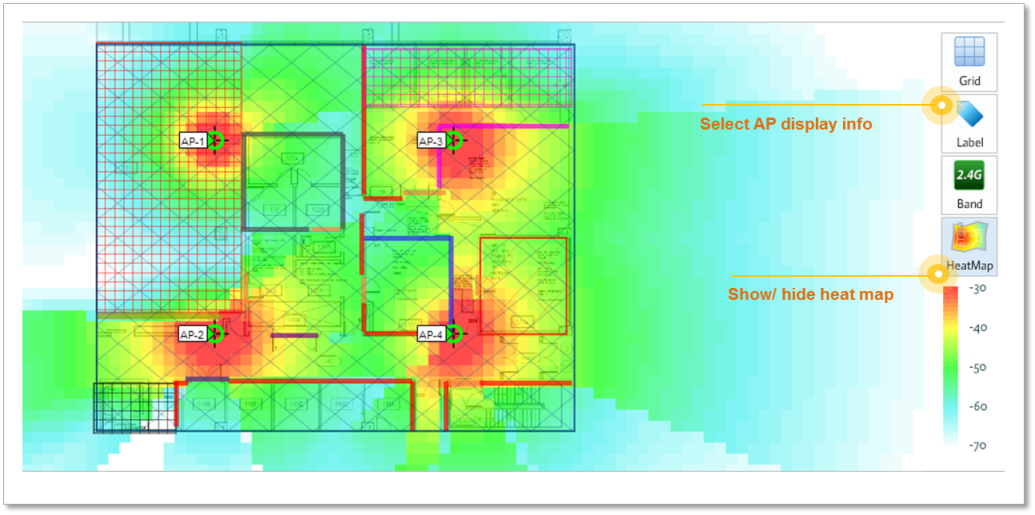
\includegraphics[scale=0.8]{./imagenes/propagacion}
\caption{Muestra software D-link sobre variación de intensidad de señal por propagación en espacio indoor.$^{\ref{fig:prop}}$}
\label{fig:propagacion}
\end{figure}

\newpage 

\textbf{Modelo de propagación}\\

Son aproximaciones matemáticas que permiten modelar el espacio físico por el cual se va a propagar la señal y que contemplan los principios físicos que la describen y que se introducen al modelo en forma de parámetros. Y que para efectos de este estudio, permiten caracterizar los valores esperados según el tipo de espacio que se vaya a caracterizar para así tener un marco de referencia con el cual contrastar las mediciones obtenidas.\\

\textit{''Estos modelos a menudo se basan en modelos probabilísticos, que pueden calcular con una cierta probabilidad de que la señal llegue o no a un determinado lugar. Algunos de estos modelos se basan en mediciones realizadas en el lugar de interés de las cuales se toman miles de mediciones que se promedian, pudiendo entonces, establecerse modelos de propagación en estos medios''}\cite{4}. De esta forma, cada modelo sirve para cada entorno, pudiendo estos a su vez, servir de base para otros modelos. Es por esto que se trabaja apoyándose tanto de información estadística como de teorías matemáticas.\\

Dado que el espacio a caracterizar, para el uso de IPS, se trata de espacios interiores, se tiene que los modelos de este tipo a aplicarse serían:\\

\textbf{Modelo de propagación Indoor}\\

Corresponden a un tipo de modelo de propagación que se adecúa a la forma en que se propagan las ondas en un espacio indoor. Contemplan fenómenos físicos como son la reflexión, la refracción y la atenuación. Estudian además, cuáles son las variantes que se adecúan mejor al espacio, es decir, si se trata de un espacio físico de varios 
pisos o de una sola planta.\\

\begin{itemize}
\item{\textbf{Modelo de propagación en espacio libre - Ecuación de FRIIS:} El modelo de propagación en espacio libre, es utilizado para estimar el nivel de potencia que se recibiría en determinado lugar cuando no se está en presencia de objetos que puedan degradar la señal, afectando la propagación de esta entre el transmisor y el receptor. Esta condición es conocida como \ac{LOS} o línea de vista.\\

Pese a lo estricto que es el tener que considerar que la señal no se propagará en un entorno con obstáculos, el modelo FRIIS es una buena referencia de comparación para enlaces de mayor complejidad. Este modelo establece que el decaimiento de la potencia es una función que depende de la distancia de separación entre el transmisor y el receptor, elevada a alguna potencia.\\

Dicha relación queda de manifiesto en la siguiente ecuación.

\begin{equation}
PL = 10\cdot{log{\left(\dfrac{P_t}{P_r}\right)}} = -10\cdot{log\left(\dfrac{\lambda^2}{(4\pi)^2\cdot{d^2}}\right)}\\
\end{equation}

donde\\

\begin{itemize}
\item{$P_t$: es la potencia transmitida, en este caso, por el router}
\item{$P_r$: es la potencia recibida, en este caso, por el equipo}
\item{$\lambda$: Es la longitud de onda a la que opera, en este caso, Wifi}
\item{$d$: Representa la distancia a la que se realiza la medición.}
\end{itemize}

De lo anterior, se tiene que la ecuación de Friis muestra, como la potencia de la señal recibida, se atenúa de acuerdo al cuadrado de la distancia entre el transmisor y el receptor. \\
}
\item{\textbf{Linear Path Attenuation Model}: Es un modelo que se usa para cuando el transmisor y el receptor se hallan en la misma planta. Las pérdidas por propagación están en dB y se obtienen a partir del \textit{path loss} en espacio libre, $PL_{FS}$, además de un factor que es lineal y que se obtiene experimentalmente.\\

Este modelo se vale de la siguiente fórmula:

\begin{equation}
PL(d) =  PL_{FS} + a\cdot{d}
\end{equation}

Donde $a$ es el coeficiente de atenuación lineal, y $d$ es la distancia entre Tx y Rx. Este coeficiente obedece a datos tabulados según el ambiente en el que se hizo la medición y que para el caso de oficinas sería de 0.47 dB/m. 
}

\item{\textbf{Modelos basados en Redes Neuronales (ANNs)}: Este tipo de modelos, recoge las imprecisiones de modelos tales como los empíricos, donde la falta de precisión es la principal deficiencia, y de modelos deterministas que si bien otorgan precisión, son altamente ineficientes, puesto que a menudo, requieren altas capacidades de procesamiento, y basándose en redes neuronales que aprovechan una base de dats de la planta en que se desea implementar, permiten con gran rapidez llegar a resultados precisos. \\

Dicha base de datos se compone de datos sobre zonas compuestas de diferentes categorías de materiales, superficies y objetos que existen en el entorno, además de la distancia entre el transmisor y el posible receptor, debiendo además, incluir información sobre el número y el tipo de materiales con que se va a encontrar la señal en las distintas categorías.\\

Las ANNs además de precisión, se valen del paralelismo sobre el cual se implementan proveyendo así una rápida evaluación de los resultados, y donde si bien, los procesos de aprendizaje suelen ser del orden de las horas, los procesos que le suceden en la predicción de niveles, es rápido.
}
\end{itemize}